\documentclass{article}

% if you need to pass options to natbib, use, e.g.:
% \PassOptionsToPackage{numbers, compress}{natbib}
% before loading nips_2016
%
% to avoid loading the natbib package, add option nonatbib:
% \usepackage[nonatbib]{nips_2016}

% \usepackage{nips_2016}

% to compile a camera-ready version, add the [final] option, e.g.:
\usepackage[final]{nips_2016}

\usepackage[utf8]{inputenc} % allow utf-8 input
\usepackage[T1]{fontenc}    % use 8-bit T1 fonts
\usepackage{hyperref}       % hyperlinks
\usepackage{url}            % simple URL typesetting
\usepackage{booktabs}       % professional-quality tables
\usepackage{amsfonts}       % blackboard math symbols
\usepackage{nicefrac}       % compact symbols for 1/2, etc.
\usepackage{microtype}      % microtypography
\usepackage{amssymb}
\usepackage{mathbbol}
\usepackage{graphicx}
\usepackage{float}


\title{10-703 - Homework 3: Deep RL and Controls}

% The \author macro works with any number of authors. There are two
% commands used to separate the names and addresses of multiple
% authors: \And and \AND.
%
% Using \And between authors leaves it to LaTeX to determine where to
% break the lines. Using \AND forces a line break at that point. So,
% if LaTeX puts 3 of 4 authors names on the first line, and the last
% on the second line, try using \AND instead of \And before the third
% author name.

\author{
  Rogerio~Bonatti\ \\
  Robotics Institute\\
  Carnegie Mellon University\\
  Pittsburgh, PA 15213 \\
  \texttt{rbonatti@andrew.cmu.edu} \\
  %% examples of more authors
  \And
  Ratnesh~Madaan\ \\
  Robotics Institute\\
  Carnegie Mellon University\\
  Pittsburgh, PA 15213 \\
  \texttt{ratneshm@andrew.cmu.edu} \\
  \And
  Adithya~Murali\ \\
  Robotics Institute\\
  Carnegie Mellon University\\
  Pittsburgh, PA 15213 \\
  \texttt{amurali@andrew.cmu.edu} \\
  %% \AND
  %% Coauthor \\
  %% Affiliation \\
  %% Address \\
  %% \texttt{email} \\
  %% \And
  %% Coauthor \\
  %% Affiliation \\
  %% Address \\
  %% \texttt{email} \\
  %% \And
  %% Coauthor \\
  %% Affiliation \\
  %% Address \\
  %% \texttt{email} \\
}

\begin{document}
% \nipsfinalcopy is no longer used

\maketitle

\begin{abstract}
  In this assignment we implemented various types of algorithms for control, including LQR, iLQR, Behavior Cloning and REINFORCE. 
\end{abstract}

\section{LQR}
Here are our results for the LQR algorithm. To run it, run the command "python run\_lqr py". Inside the "run lqr\_py" script the user can change the type of environment.

\subsection{[5pts] Test your LQR implementation on the TwoLinkArm-v0 environment. Record the total reward and number of steps to reach the goal. Also plot $q$, $\dot{q}$, and your control inputs $u$}

num\_steps=135
reward=-313.459702915

\begin{figure}[H] \label{fig:lqr_qn1}
  \centering
  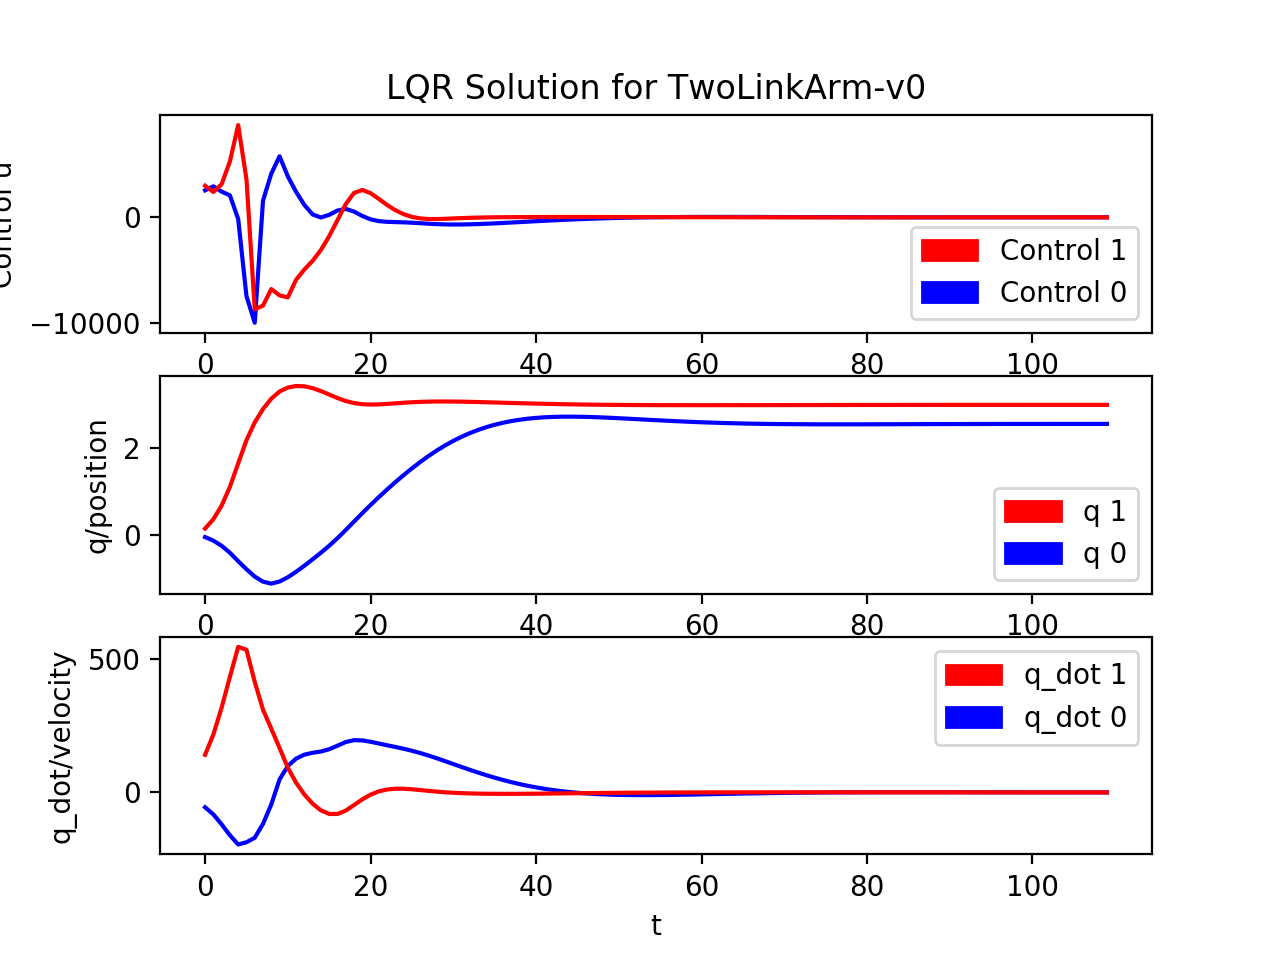
\includegraphics[width=1.2\textwidth]{images/lqr_qn1}
  \caption{Plots for LQR q1}
\end{figure}

\subsection{[5pts] Test your LQR implementation on the TwoLinkArm-limited-torque-v0 environment. Record the total reward and the number of steps to reach the goal. Also plot $q$, $\dot{q}$, and your control inputs $u$. Additionally plot u clipped to the action space of this environment.}

num\_steps=2682, reward=-8912.41442527

\begin{figure}[H] \label{fig:lqr_qn2}
  \centering
  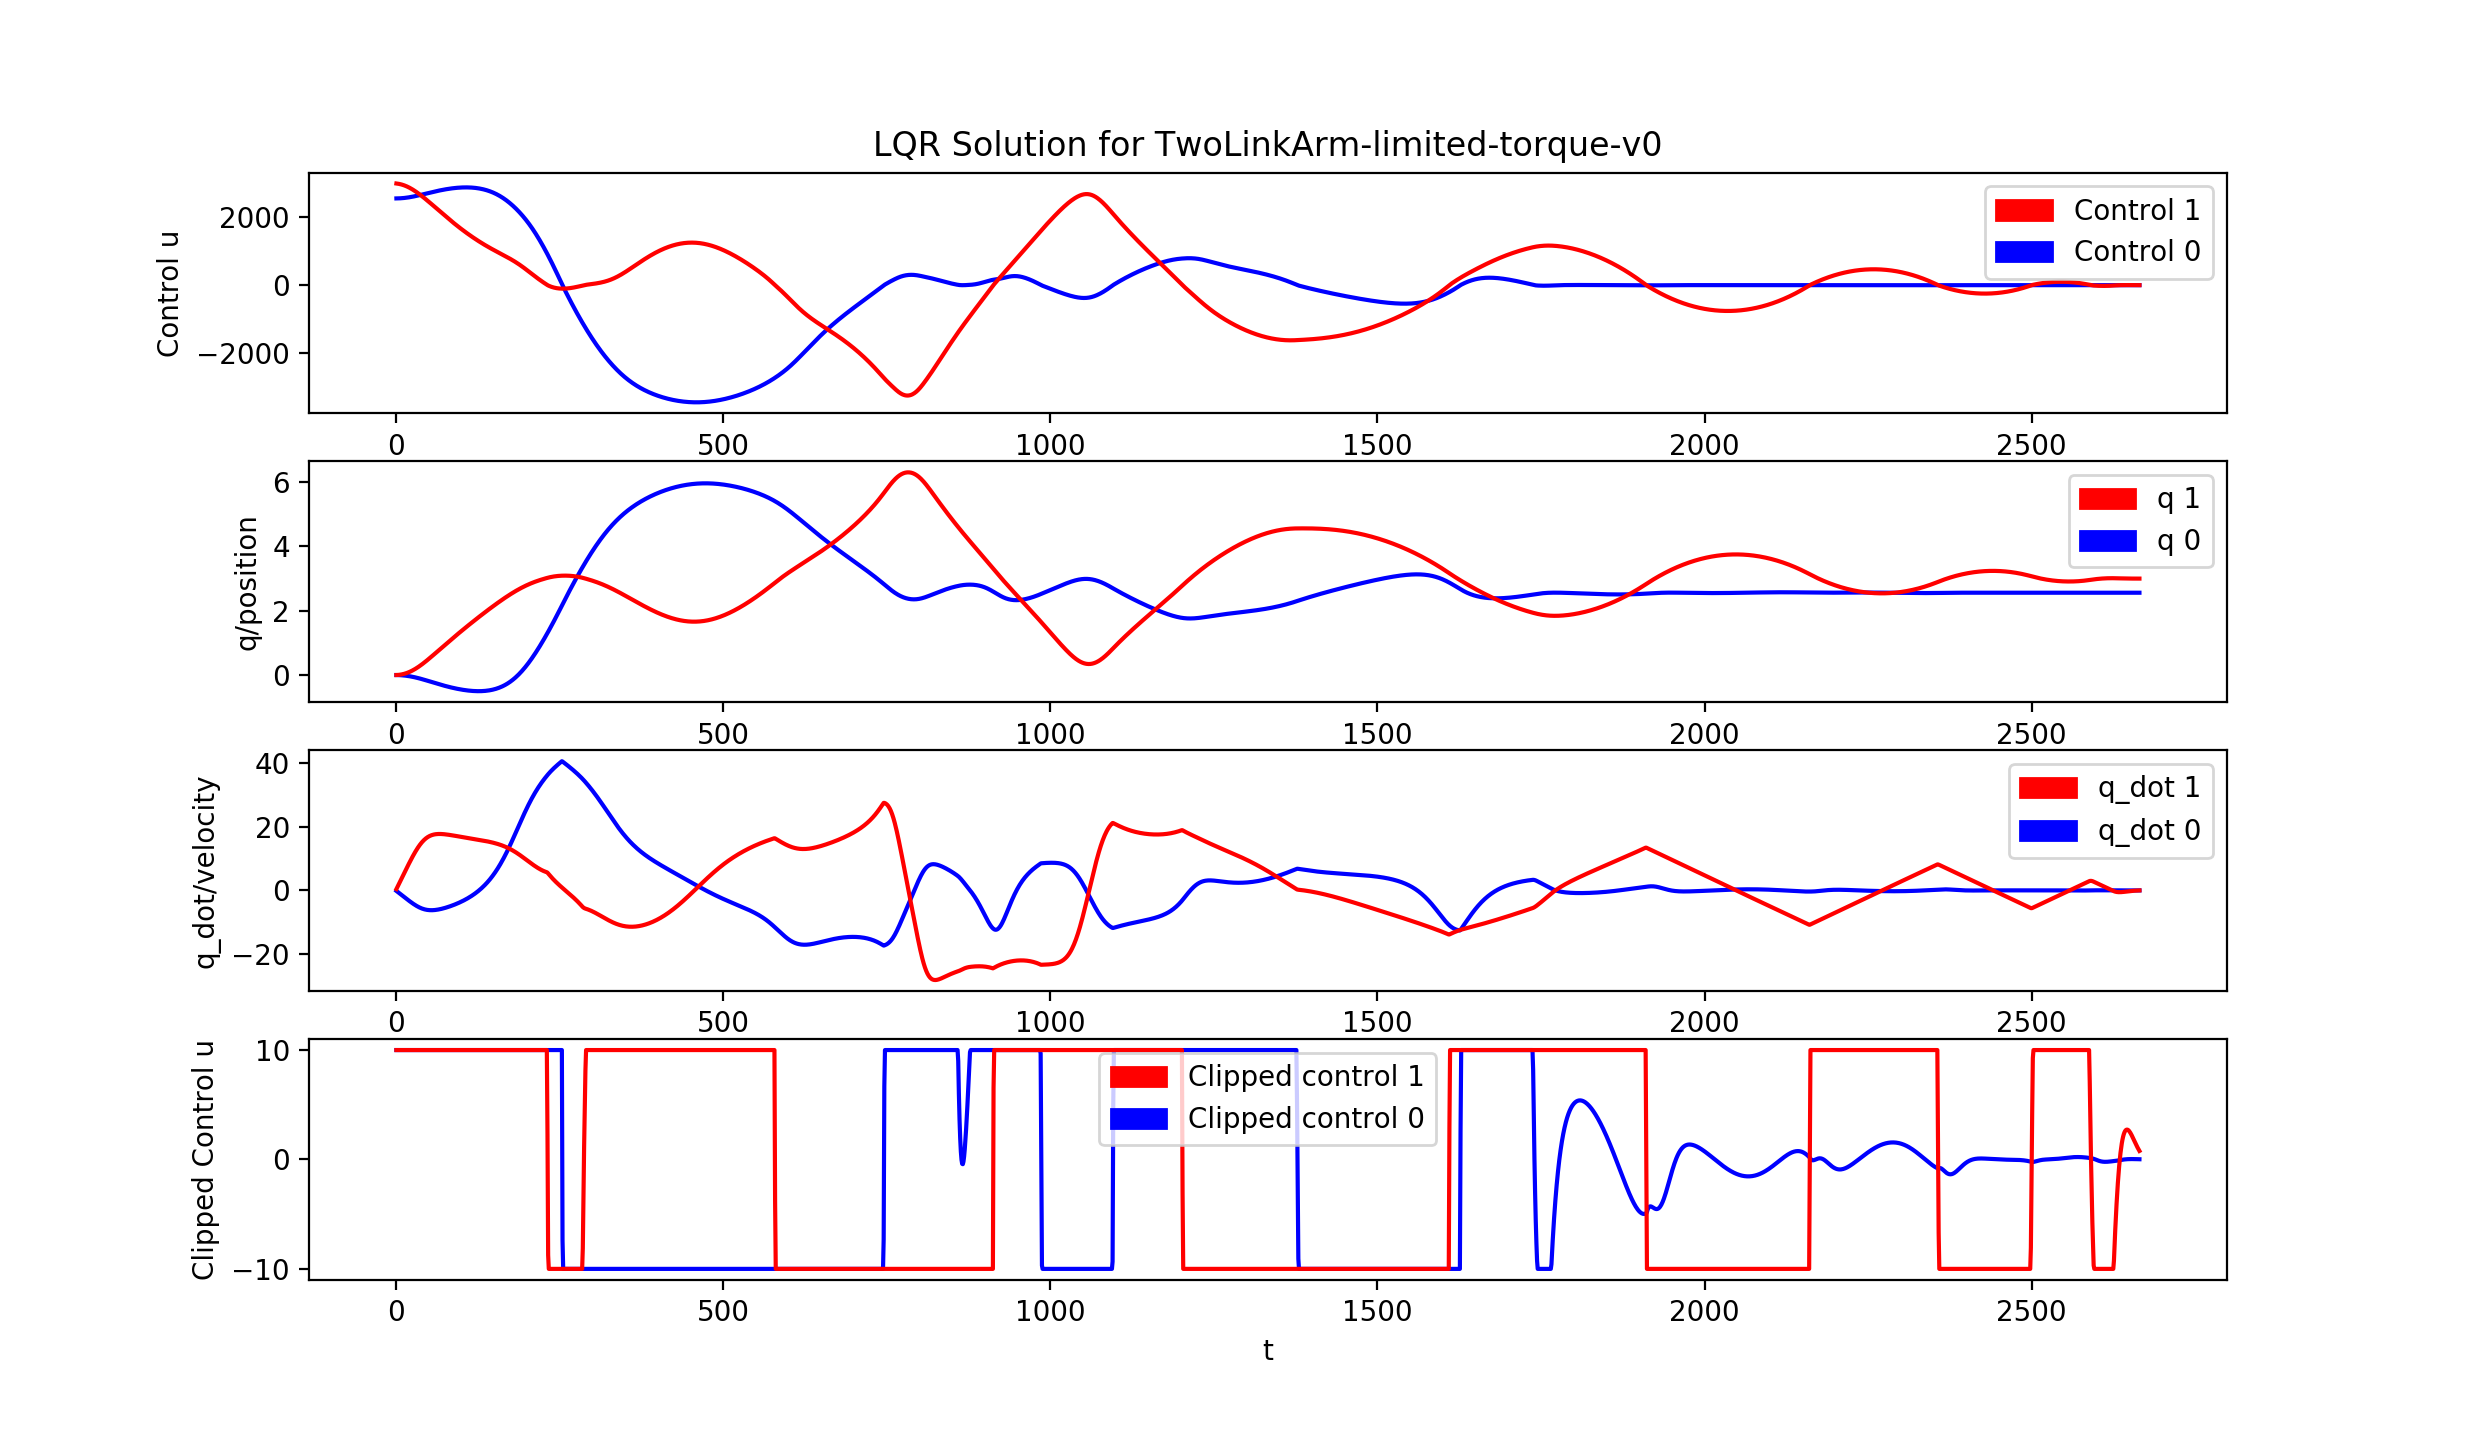
\includegraphics[width=1.2\textwidth]{images/lqr_qn2}
  \caption{Plots for LQR q2}
\end{figure}

\subsection{[5pts] Compare the performance of your controller on each of these environments}

In the unlimited torque environment the controller was able to stabilize the arm in a much shorter time than in the limited torque environment (t=40 versus t=2500). This happened because the system was able to impose extremely high torques to the arm to first move it closer to the desired position, and later de-accelerate the arm so that it remained stationary. The downside is that these very high torques are not feasible in real-life systems. 

A possible way to maintain the torques within the acceptable range in a real-life system would be to penalize high torques more in the cost function, increasing the value of components in matrix R.


\subsection{[5pts] Test your LQR implementation on the TwoLinkArm-v1 environment. Record the total reward and number of steps to reach the goal. Also plot $q$, $\dot{q}$, and your control inputs $u$}

num\_steps=621, reward=-1788.50332694

\begin{figure}[H] \label{fig:lqr_qn4}
  \centering
  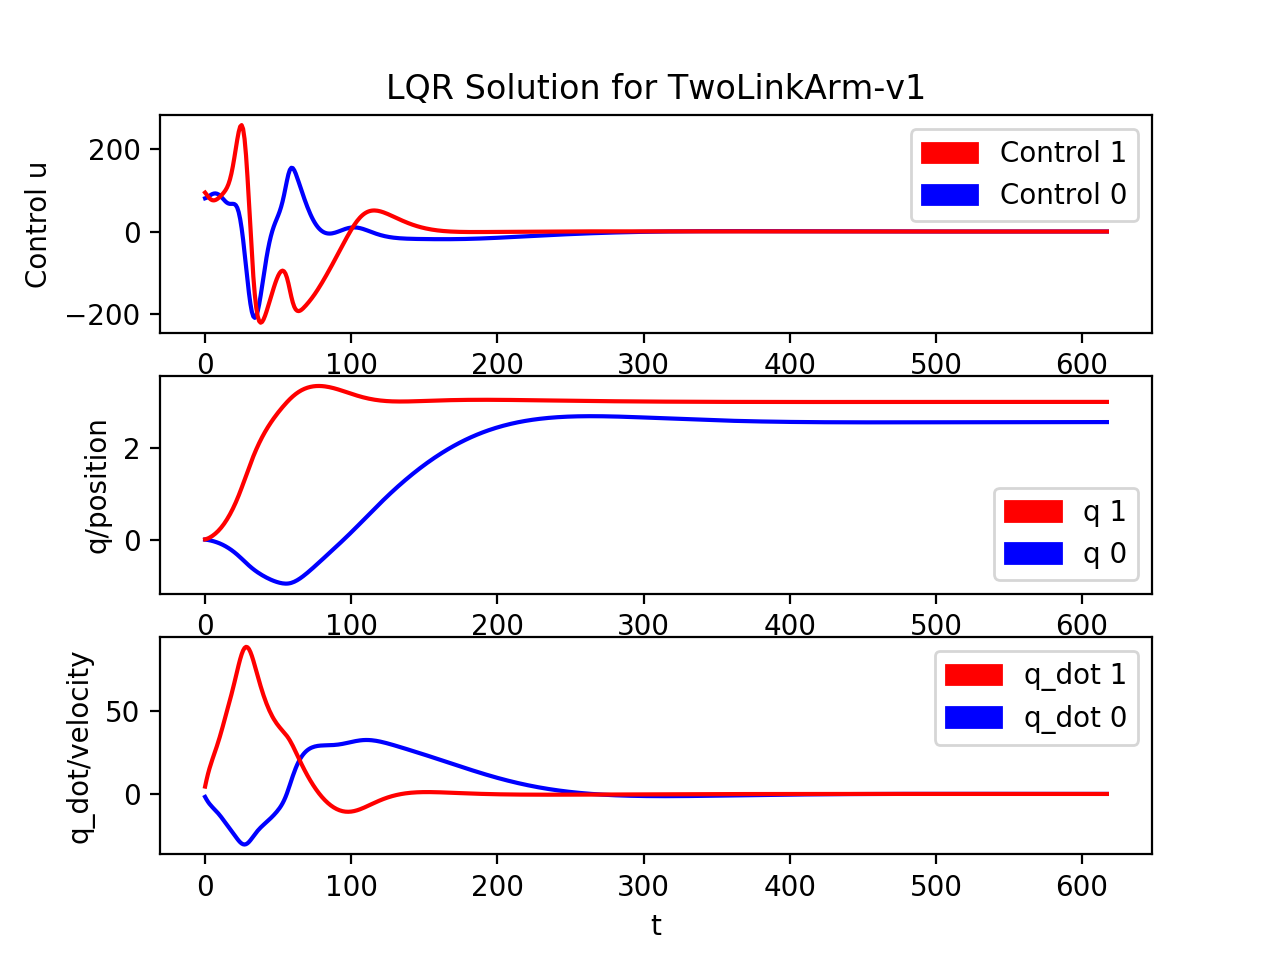
\includegraphics[width=1.2\textwidth]{images/lqr_qn4}
  \caption{Plots for LQR q4}
\end{figure}

\subsection{[5pts] Test your LQR implementation on the TwoLinkArm-limited-torque-v1 environment. Record the total reward and the number of steps to reach the goal. Also plot $q$, $\dot{q}$, and your control inputs $u$. Additionally plot u clipped to the action space of this environment.}

num\_steps=1190, reward=-2704.41159978

\begin{figure}[H] \label{fig:lqr_qn5}
  \centering
  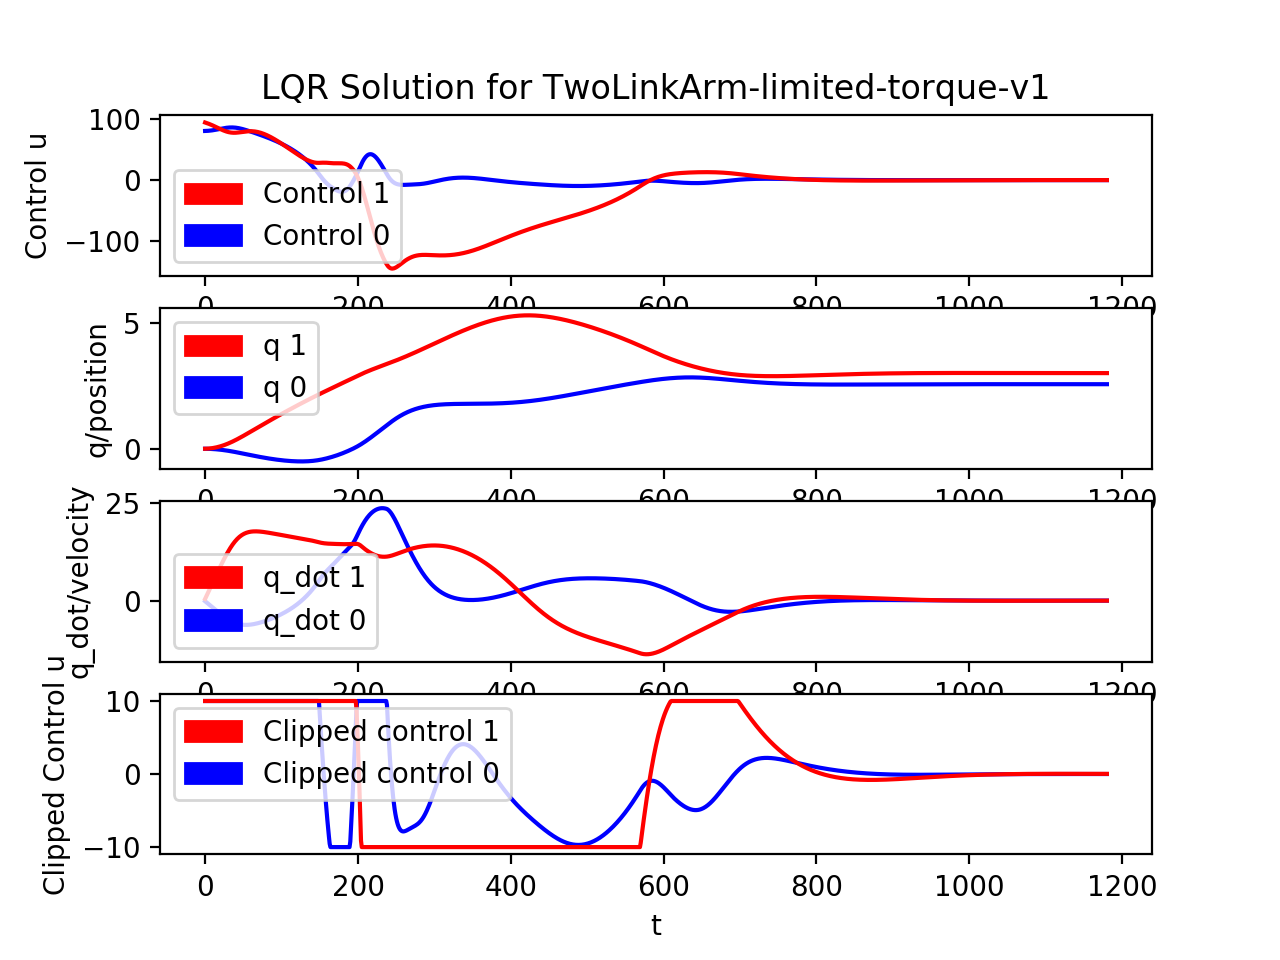
\includegraphics[width=1.2\textwidth]{images/lqr_qn5}
  \caption{Plots for LQR q5}
\end{figure}

\subsection{[5pts] Compare the performance on these environments to the v0 versions.}

The positions obtained in the v1 environments took longer to stabilize than positions in the v0 environment because the torques applied in the v1 system were significantly smaller (around 200 max control versus 10000 max control). This happened because the cost function in the v1 (matrix R) environment penalizes high torques much more heavily than in v0, therefore lower torques are preferred. Despite the slower convergence, both systems were able to reach the end position without much oscillatory behavior.


\section{iLQR}
Here are our results for the iLQR algorithm. To run it, run the command "python run\_ilqr.py". Inside the "run\_ilqr.py" script the user can change the type of environment. 
A reference for our code was the StudyWolf blog, available at https://studywolf.wordpress.com/2016/02/03/the-iterative-linear-quadratic-regulator-method/

\subsection{[10pts] Test your iLQR implementation on the TwoLinkArm-v0 environment. Plot the total cost (intermediate cost + final cost) respect to iterations and record the total reward. Also plot $q$, $\dot{q}$, and your control inputs $u$.}

reward=-333.314787036

\begin{figure}[H] \label{fig:ilqr_qn1}
  \centering
  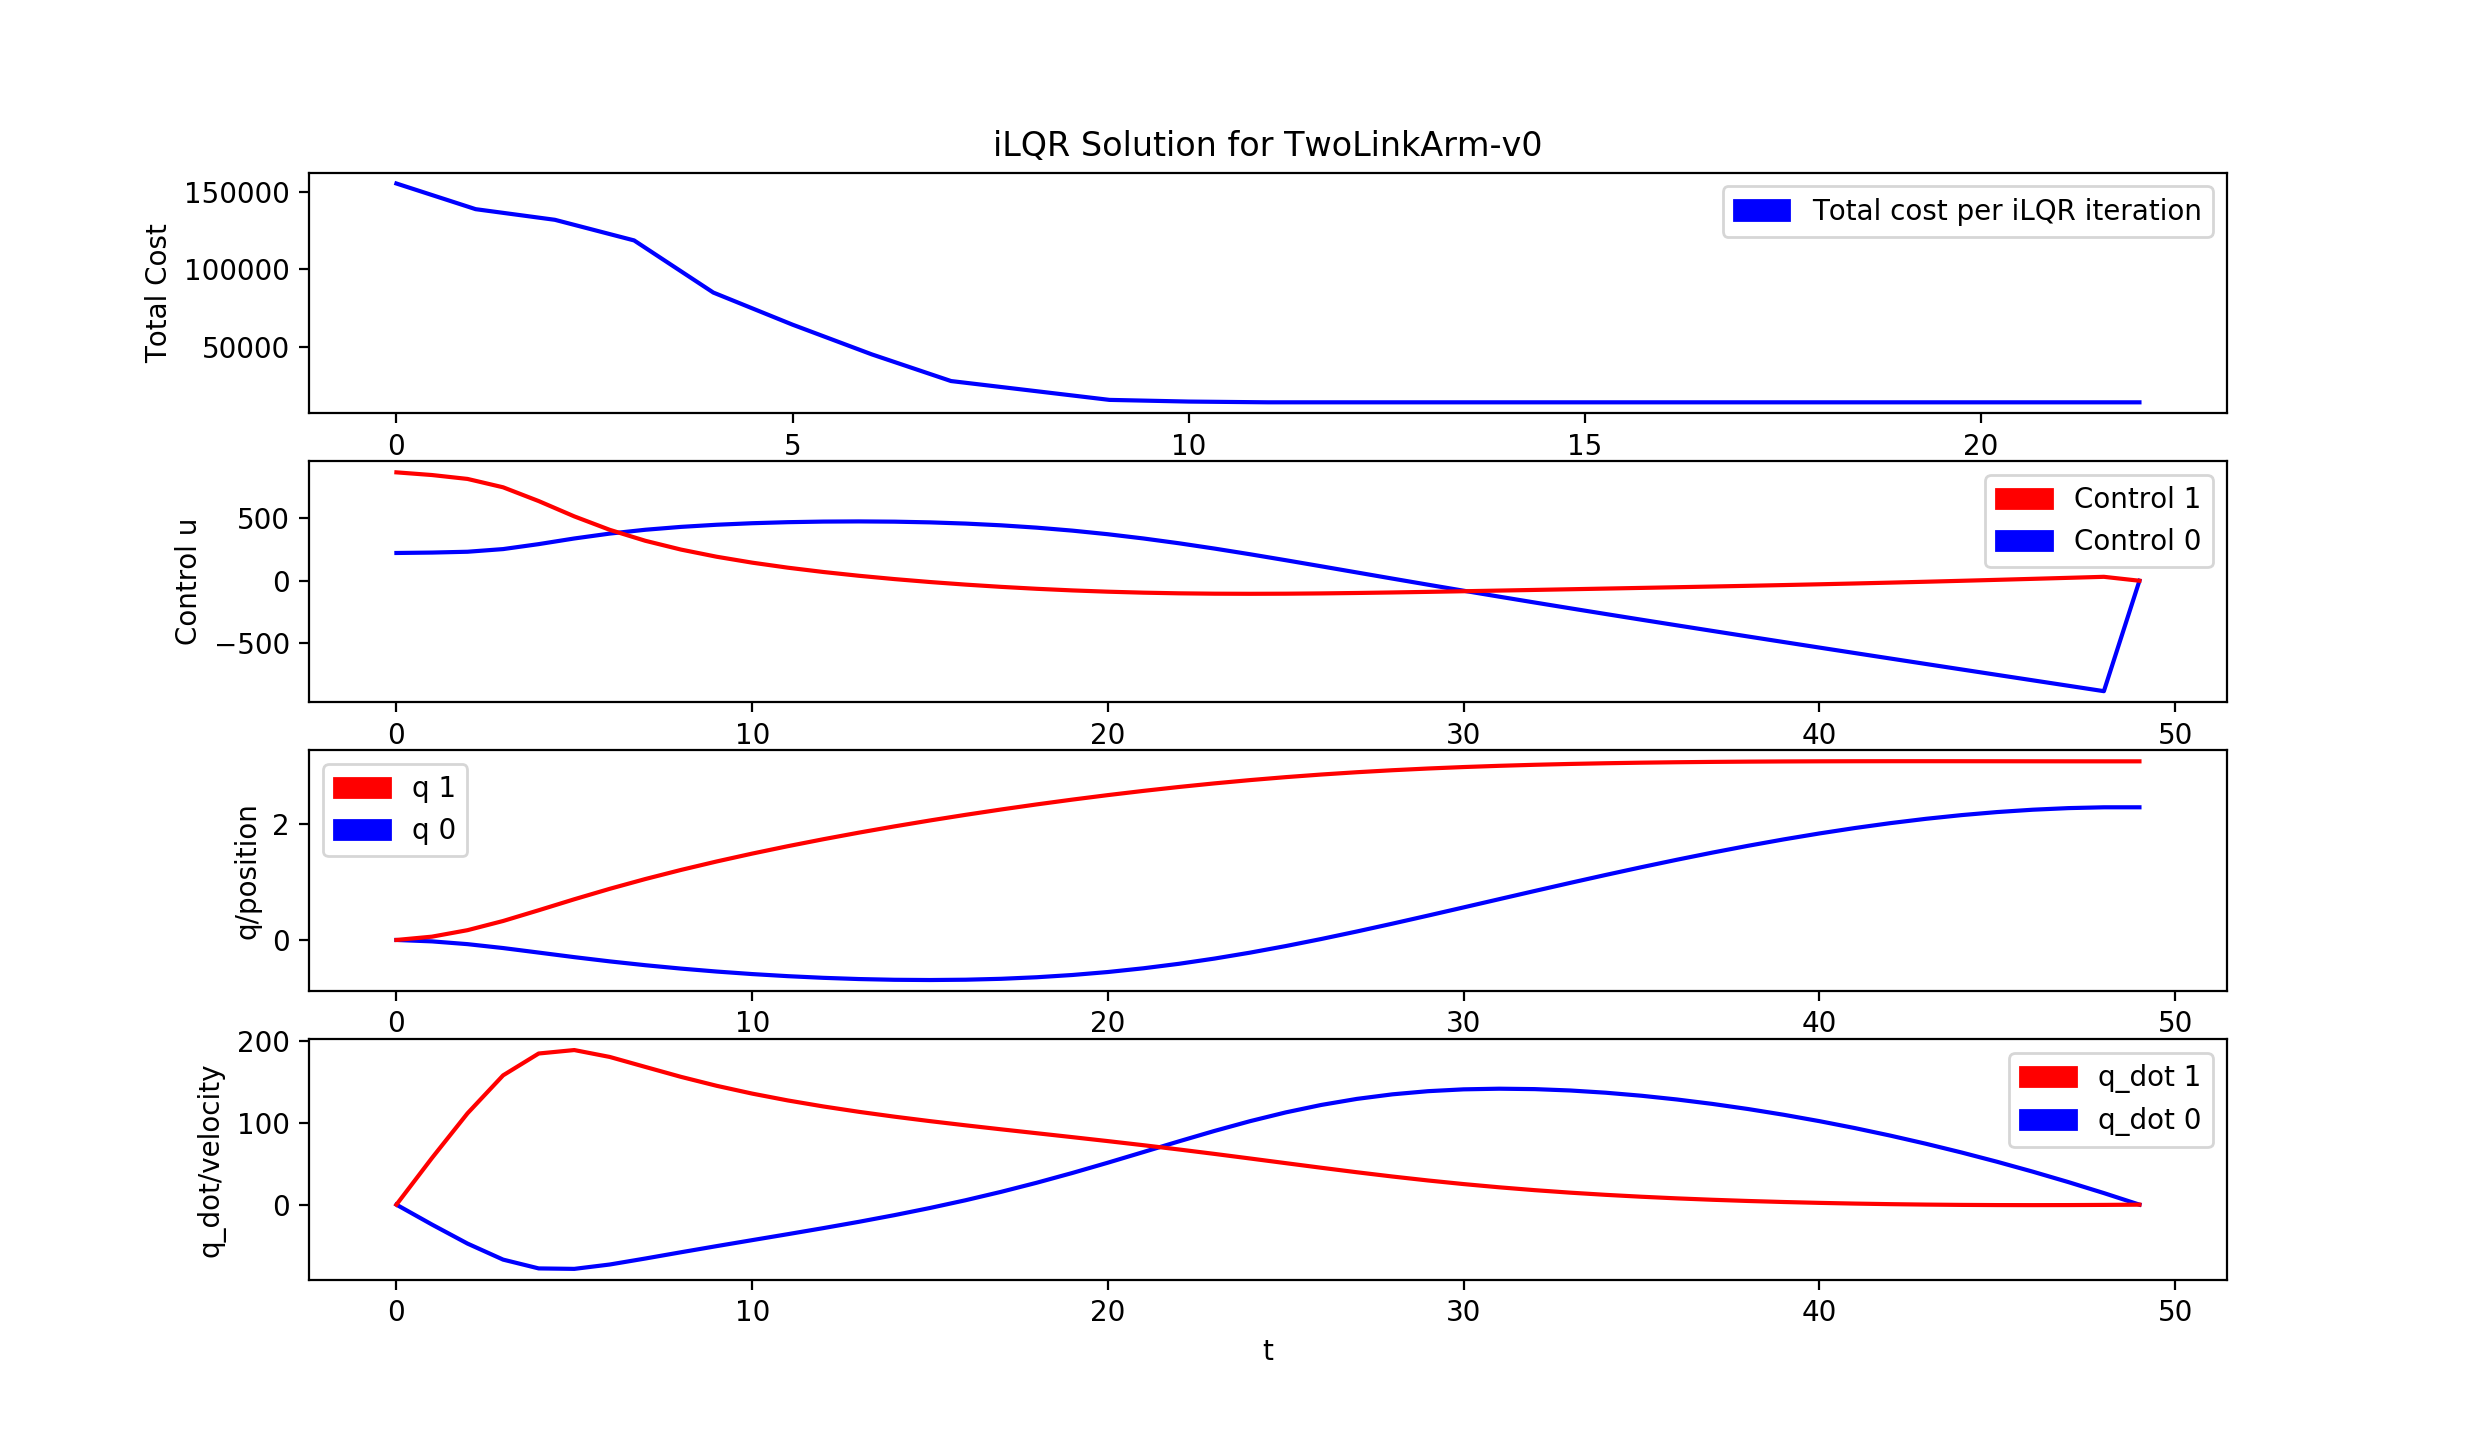
\includegraphics[width=1.2\textwidth]{images/ilqr_qn1}
  \caption{Plots for iLQR q1}
\end{figure}

\subsection{[10pts] Test your iLQR implementation on the TwoLinkArm-v1 environment. Plot the total cost (intermediate cost + final cost) respect to iterations and record the total reward. Also plot $q$, $\dot{q}$, and your control inputs $u$.}

reward=-14352.1694183

\begin{figure}[H] \label{fig:ilqr_qn2}
  \centering
  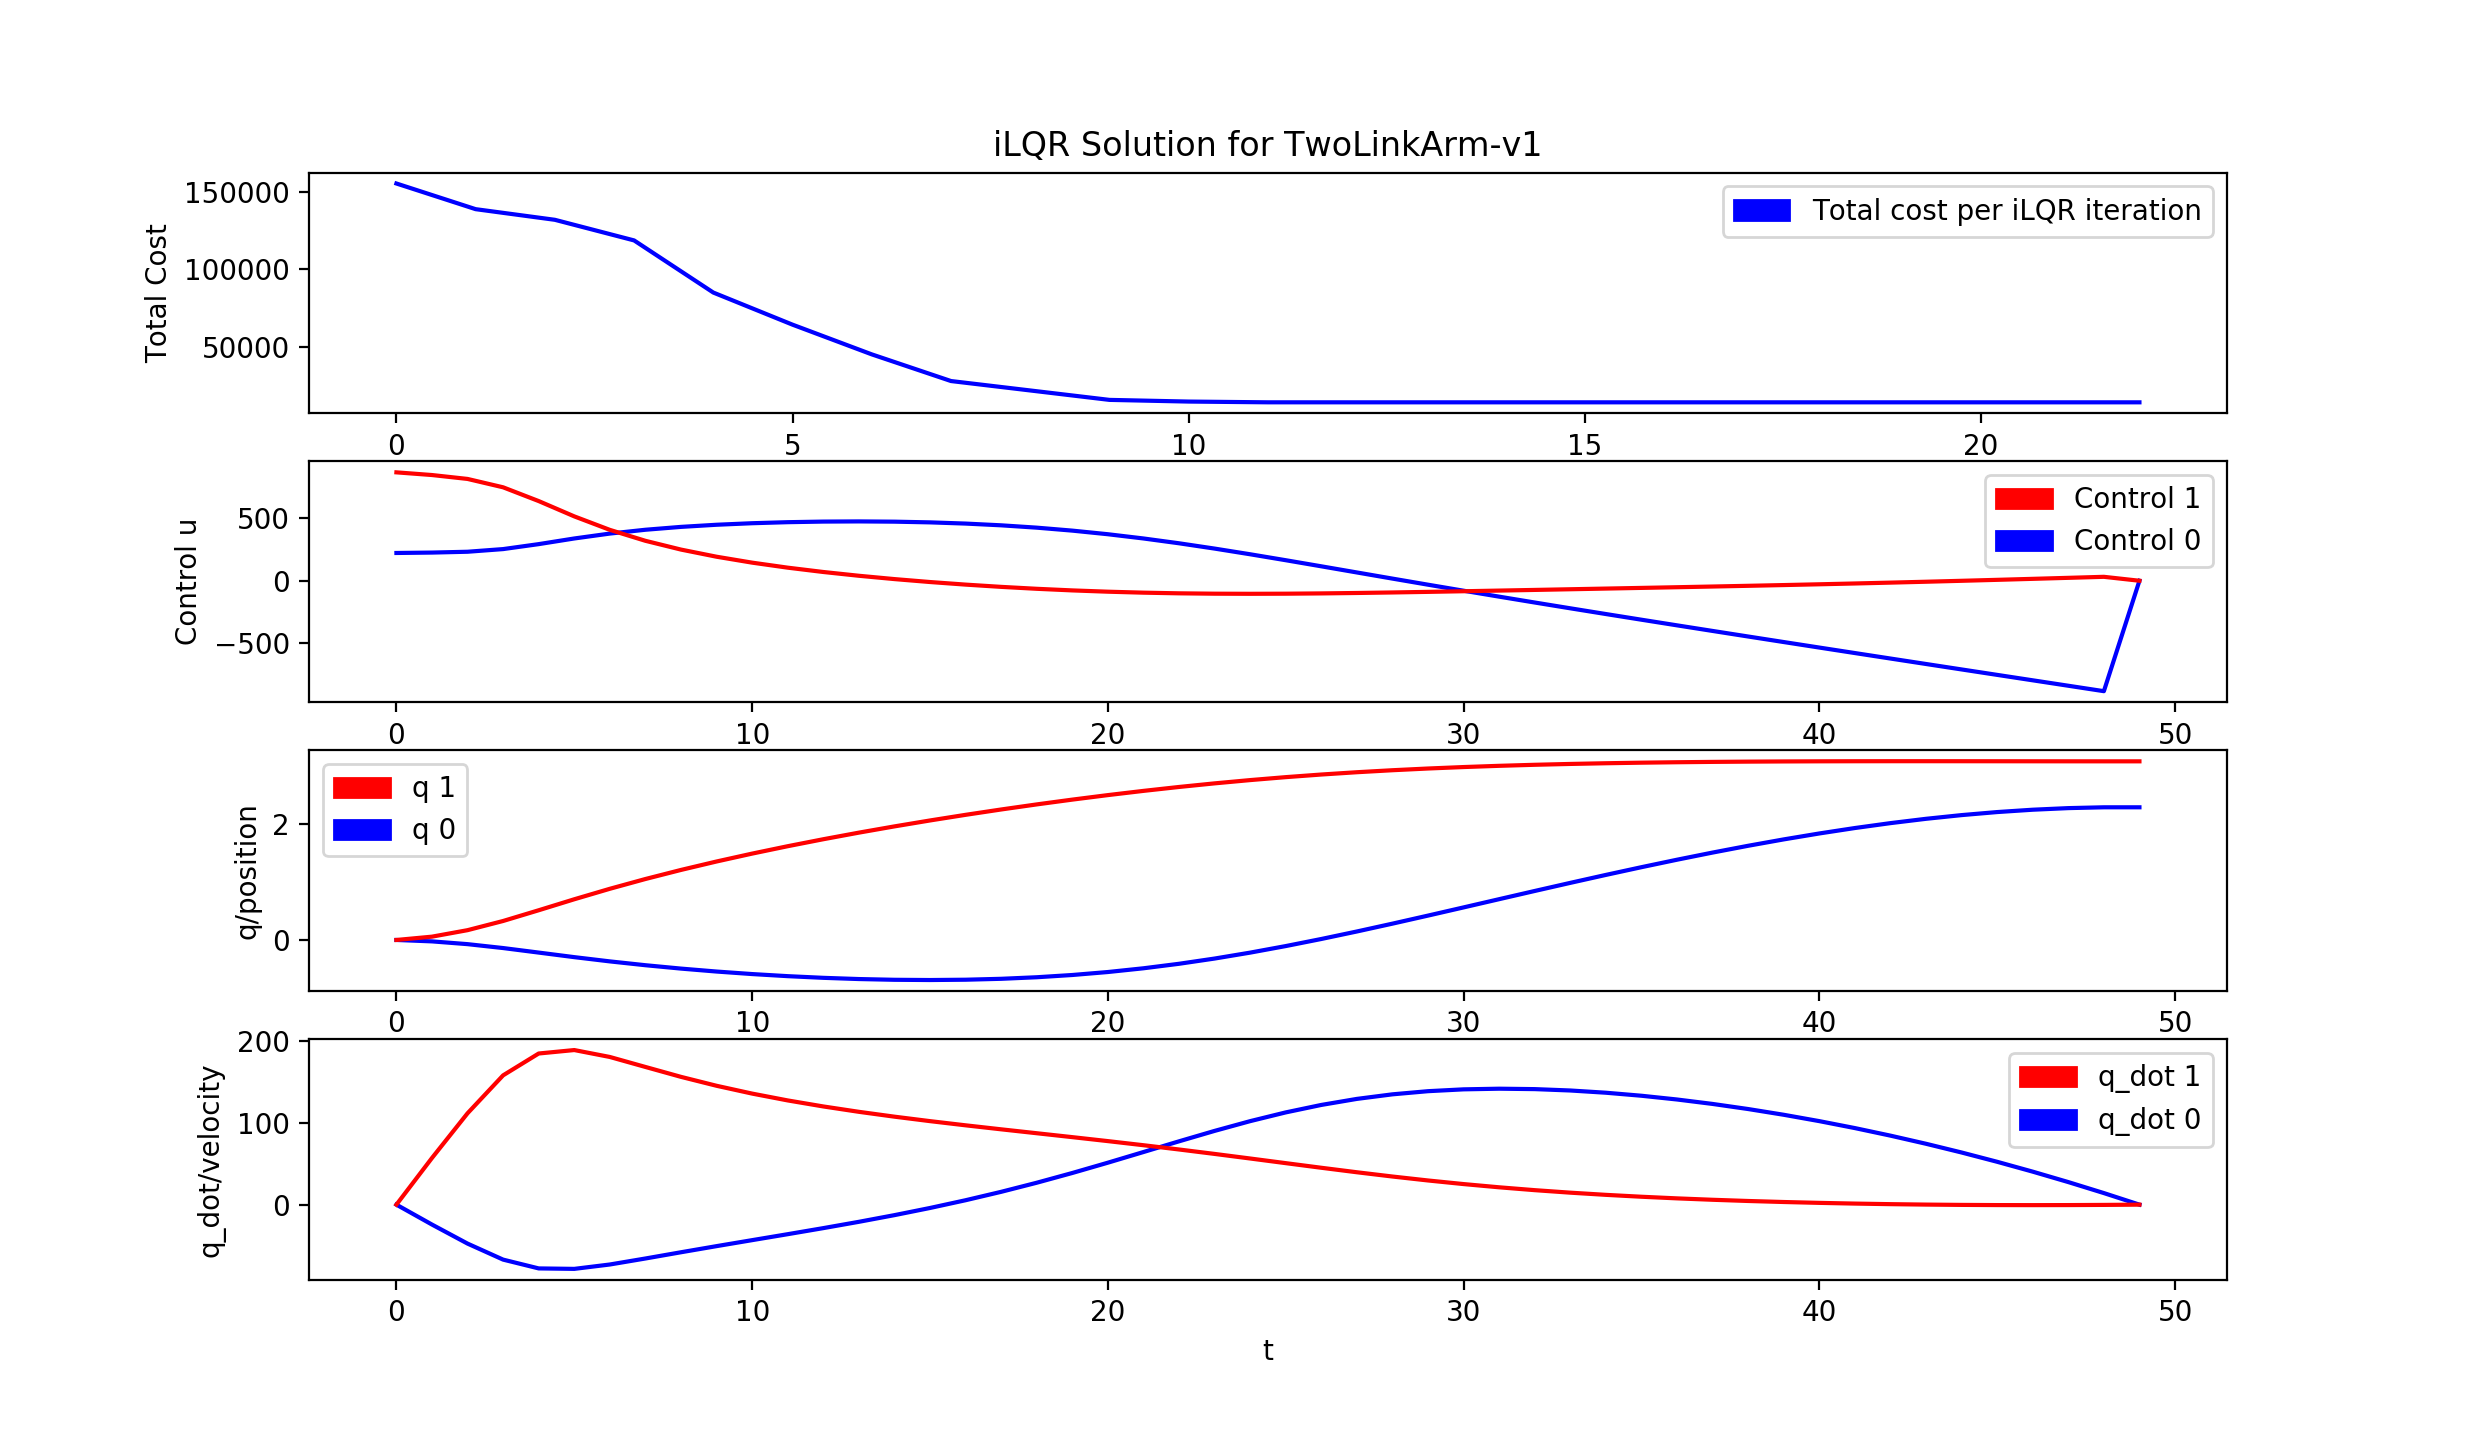
\includegraphics[width=1.2\textwidth]{images/ilqr_qn2}
  \caption{Plots for iLQR q2}
\end{figure}

\subsection{[5pts] Discuss the comparison between iLQR and LQR algorithm, which one is better and why?}

The iLQR algorithm is definitely better than the LQR algorithm. This is because the end position of the arm was achieved in about the same time using both algorithms (around t=40), but iLQR used a significantly lower torque to achieve the objective (max torque at about 1000 versus 10000), and presented much smoother movements, without oscillatory behavior. This happens because iLQR predicts the future dynamics of the system in its movements. The downside is the increase in computational time.

\subsection{[5pts EXTRA CREDIT] iLQR is not as fast as we want. Try to improve the convergence in any way you can figure out. Potential directions include changing cost function and use better optimization procedures.}

We can change the intermediate cost function of iLQR to instead of just penalizing for applying a high control torque, penalize the system for not being close to our final objective. 



\section{Behavior cloning}
Here are our results for the behavior cloning algorithm. 

\subsection{[10pts] Use each of your datasets to train a cloned behavior using the dataset as a supervised learning problem. Record the final loss and accuracy of your model after training for at least 50 epochs. Make sure you include any hyper parameters in your report}

\begin{table}[H]
\centering
\caption{Results}
\label{my-label}
\begin{tabular}{ccc}
\textbf{No of episodes} & \textbf{Loss}  & \textbf{Accuracy} \\
1                       & 0.280591886044 & 0.8650    \\
10                     & 0.104798256934 & 0.9575   \\
50                     & 0.0489679535789 & 0.9815   \\
100                   & 0.0508819897211 & 0.9786
\end{tabular}
\end{table}


\begin{table}[H]
\centering
\caption{Hyperparams}
\label{my-label2}
\begin{tabular}{cc}
Optimizer  & 'Adam'                 \\
Loss       & 'binary\_crossentropy' \\
Batch size & 32                     \\
Epochs     & 50                    
\end{tabular}
\end{table}


\subsection{[[10pts] Evaluate each of your cloned models on the CartPole-v0 model using the test cloned policy method. How does the amount of training data affect the cloned policy?}

\begin{table}[H]
\centering
\caption{Results on normal environment}
\label{my-label3}
\begin{tabular}{ccc}
No of episodes & Mean reward & Standard deviation \\
1              & 127.22       & 63.24    \\
10            & 200.00       & 0.00      \\
50            & 200.00       & 0.00    \\
100          & 200.00       & 0.00     
\end{tabular}
\end{table}

Expert:
Mean reward : 200.0
Std : 0.0

If we train on only single episode, the cloned policy performs poorly. However, for all the other three cases, the cloned policy exhibits the optimal performance regardless of the amount of training data used. 

\subsection{[10pts] Evaluate each of your cloned models on the CartPole-v0 domain wrapped with the wrap cartpole function. Also evaluate the expert policy. How does your cloned behavior compare with respect to the expert policies and each other.}

\begin{table}[H]
\centering
\caption{Results on noisy environment}
\label{my-label4}
\begin{tabular}{ccc}
No of episodes & Mean reward & Standard deviation \\
1            & 13.88       & 9.33946465275      \\
10           & 64.94       & 56.4508317034      \\
50           & 75.40       & 72.7403601861      \\
100          & 77.04       & 77.6193171833      
\end{tabular}
\end{table}

Expert:
Mean reward : 70.58
Std : 46.62

As episode length increases, the mean reward increases along with standard devaition. 
Cloned models trained on 50 and 100 episodes do better than the expert, however with a greater amount of standard deviation of the reward. 




\section{REINFORCE}

\subsection{[10pts] Train REINFORCE on CartPole-v0 until convergence. Show your learning curves for the agent. In other words, every k episodes, freeze the current cloned policy and run 100 test episodes. Average the total reward and track the min and max reward. Plot the total reward on the y-axis with min/max values as error-bars vs the number of training episodes.}

Below are the training results. We use the provided Keras model architecture and train using the Adam Optimizer with a learning rate of $0.00025$. The policy is evaluted for 100 episodes every 20 training episodes. The average reward is plotted along with the minimum and maximum for every 100 test episodes.

The instability is largely due to the overcomplicated model architecture. A simple one layer network trains in many less episodes with better performance.
\begin{center}
  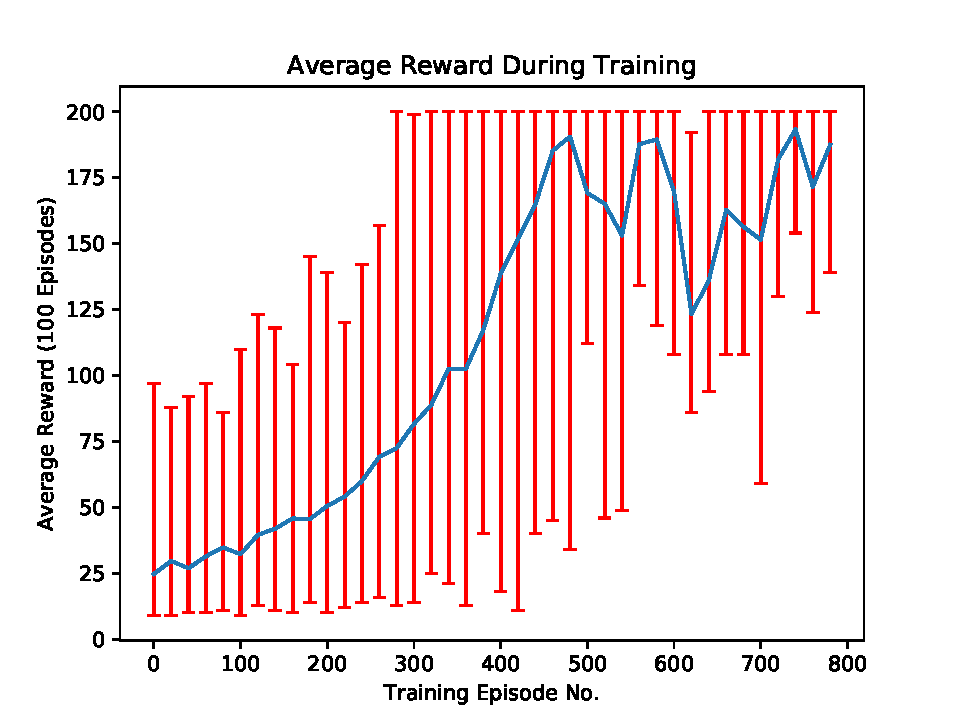
\includegraphics[width=12cm]{images/reinforce_plot.pdf}
\end{center}

\subsection{[10pts] How does this policy compare to our provided expert and your cloned models?}

Although this policy can achieve a perfect episode of 200 reward, it is not as stable as the provided expert nor the cloned models when evaluated on the default CartPole-v0 environment. Since the policy is stochastic, it can exhibit poor performance as evalauted during training. If the policy was followed deterministically (by using an argmax) the reward will likely have less variance and stay closer to a reward of 200. More iterations of REINFORCE, perhaps with a decaying gradient descent step size, as well as adding a baseline state value function, might reduce the variance over time.

% \section*{References}

\small
\medskip
\bibliographystyle{plain}
\bibliography{bibliography}


\end{document}
